% Ficha del proyecto Astro Granja (ES/EN) - NASA Space Apps Challenge 2026, Sangolquí
% Plantilla tipo "data sheet": banda de encabezado, tarjetas (tcolorbox) y tablas de fuentes.
% Compilar con pdfLaTeX:  pdflatex ficha.tex
\documentclass[10pt,a4paper]{article}
\usepackage[margin=1.6cm,top=1.3cm,bottom=1.6cm]{geometry}
\usepackage[T1]{fontenc}
\usepackage[utf8]{inputenc}
\usepackage[scaled=0.95]{helvet}
\renewcommand{\familydefault}{\sfdefault}
\newcommand{\titulo}{\bfseries}
\usepackage[english,spanish,es-noshorthands]{babel}
\usepackage{microtype}
\usepackage{xcolor}
\usepackage{graphicx}
\usepackage{tabularx,booktabs,array}
\usepackage{tcolorbox}
\usepackage{enumitem}
\usepackage{fancyhdr}
\usepackage{hyperref}

\definecolor{tierra}{HTML}{4B2612}
\definecolor{verde}{HTML}{2E6B1F}
\definecolor{rojo}{HTML}{C8372D}
\definecolor{azul}{HTML}{1E5A8C}
\definecolor{crema}{HTML}{FBF1E0}
\definecolor{oro}{HTML}{F2B33D}
\hypersetup{colorlinks=true,urlcolor=azul,linkcolor=azul,pdftitle={Astro Granja - Ficha del proyecto / Project fact sheet},pdfauthor={Aquarela Team}}

\setlength{\parindent}{0pt}
\setlength{\parskip}{3pt}
\setlist{nosep,leftmargin=1.2em}
\renewcommand{\arraystretch}{1.25}

\pagestyle{fancy}\fancyhf{}
\renewcommand{\headrulewidth}{0pt}
\fancyfoot[L]{\footnotesize\color{tierra!70}Astro Granja · Aquarela Team · NASA Space Apps Challenge 2026 · Sangolquí}
\fancyfoot[R]{\footnotesize\color{tierra!70}\thepage}

% Banda de encabezado
\newcommand{\banda}[3]{%
\begin{tcolorbox}[colback=verde,colframe=oro,boxrule=0pt,bottomrule=4pt,arc=6pt,left=12pt,right=12pt,top=10pt,bottom=10pt,
  fontupper=\color{white}]
{\titulo\fontsize{26}{28}\selectfont #1}\\[2pt]
{\large #2}\\[4pt]
{\small #3}
\end{tcolorbox}}

% Tarjeta con título
\newtcolorbox{tarjeta}[2][verde]{colback=crema,colframe=#1,arc=5pt,boxrule=1.2pt,
  title={\bfseries #2},coltitle=white,colbacktitle=#1,fonttitle=\large,left=8pt,right=8pt,top=5pt,bottom=5pt,
  before skip=6pt,after skip=6pt}

\newcommand{\enlace}[2]{\href{#1}{#2}}

\begin{document}

%=============================== ESPAÑOL ===============================
\banda{Astro Granja}{Ficha del proyecto · Juego para niños con datos reales de la NASA}%
{Equipo \textbf{Aquarela Team} · Reto \textbf{Field Shift: Adapting Farms with NASA Data} · NASA Space Apps Challenge 2026 · Sangolquí (ESPE), Ecuador}

\begin{tarjeta}{Resumen}
\textbf{Astro Granja} es un juego web para niños de 8 a 12 años de la sierra ecuatoriana. Pachita, una granjera andina, llega en cohete
y enseña a elegir una parcela real en el mapa, leer su clima con datos de la NASA, sembrar cultivos andinos en su época, regar cuando la
tierra tiene sed y \textbf{rotar con leguminosas} para que el suelo no se canse. Todo número del juego sale de NASA POWER procesado con
FAO-56; nada es inventado. Funciona en el celular, en español e inglés, y con un modo sin 3D para teléfonos sencillos.
\end{tarjeta}

\begin{tarjeta}[azul]{1. Datos de la NASA usados (nombre, enlace y uso)}
\small
\begin{tabularx}{\linewidth}{@{}>{\raggedright\arraybackslash}p{3.6cm} >{\raggedright\arraybackslash}p{4.2cm} X@{}}
\toprule
\textbf{Dataset / API} & \textbf{Variables} & \textbf{Uso en el juego} \\
\midrule
\enlace{https://power.larc.nasa.gov/docs/services/api/temporal/daily/}{NASA POWER Daily API} (comunidad AG, 2001–2024) &
\texttt{PRECTOTCORR}, \texttt{T2M\_MAX}, \texttt{T2M\_MIN}, \texttt{RH2M}, \texttt{WS2M}, \texttt{ALLSKY\_SFC\_SW\_DWN} &
Clima real de cada día del juego, rango de lluvia (año seco, normal, lluvioso), días de calor y evaporación FAO-56 Penman-Monteith. \\
\enlace{https://power.larc.nasa.gov/docs/services/api/temporal/climatology/}{NASA POWER Climatology API} &
\texttt{GWETROOT}, \texttt{GWETTOP} &
Humedad del suelo en las raíces mes a mes: barras de la ficha “Así es tu tierra” y meses en que hay que regar. \\
\enlace{https://gmao.gsfc.nasa.gov/reanalysis/MERRA-2/}{MERRA-2} (NASA GMAO) &
Base de temperatura, humedad, viento y humedad del suelo de POWER &
Fuente de los parámetros meteorológicos de POWER. \\
\enlace{https://ceres.larc.nasa.gov/}{CERES} (NASA LaRC) &
Radiación solar en superficie &
Fuente de \texttt{ALLSKY\_SFC\_SW\_DWN} (energía del sol por día). \\
\enlace{https://gpm.nasa.gov/data/imerg}{GPM IMERG} &
Lluvia &
Fuente de la lluvia corregida \texttt{PRECTOTCORR} de POWER. \\
\bottomrule
\end{tabularx}
\vspace{2pt}
{\footnotesize Consulta usada (código en \texttt{app/clients.py}):\\
\texttt{power.larc.nasa.gov/api/temporal/daily/point?parameters=T2M\_MAX,T2M\_MIN,PRECTOTCORR,}\\
\texttt{RH2M,WS2M,ALLSKY\_SFC\_SW\_DWN\&community=AG\&start=20010101\&end=20241231\&latitude=\ldots}}\\
Atribución: datos obtenidos del NASA Langley Research Center (LaRC) POWER Project, financiado por el NASA Earth Science/Applied Science Program.
\end{tarjeta}

\begin{tarjeta}[tierra]{Fuentes complementarias (no son de la NASA)}
\small
\textbf{FAO-56} (\enlace{https://www.fao.org/4/x0490e/x0490e00.htm}{Allen et al., 1998}): evapotranspiración y coeficientes de cultivo ·
\textbf{INIAP}: épocas de siembra y cultivos andinos ·
\textbf{INAMHI}: validación con 85 estaciones ·
\textbf{Open-Meteo} (\enlace{https://open-meteo.com/}{open-meteo.com}): corrección por altura con ECMWF IFS 9 km y relieve Copernicus DEM ·
\textbf{Esri World Imagery}: fondo del mapa.
\end{tarjeta}

\begin{tarjeta}[verde]{2. Repositorio y licencia · 3. Enlaces}
\small
\begin{tabularx}{\linewidth}{@{}>{\bfseries}p{4.1cm} X@{}}
Juego desplegado (demo) & \enlace{https://pacha-chat.vercel.app}{pacha-chat.vercel.app} \\
Repositorio público & \enlace{https://github.com/M47H3W1/pacha-bot}{github.com/M47H3W1/pacha-bot} \\
Licencia (raíz del repo) & \enlace{https://github.com/M47H3W1/pacha-bot/blob/develop/LICENSE}{MIT License — LICENSE} \\
Capturas de pantalla & \enlace{https://github.com/M47H3W1/pacha-bot/tree/develop/docs/entregables/capturas}{docs/entregables/capturas} \\
Presentaciones (PDF) & \enlace{https://github.com/M47H3W1/pacha-bot/blob/develop/docs/entregables/Presentacion_ES.pdf}{Español} ·
\enlace{https://github.com/M47H3W1/pacha-bot/blob/develop/docs/entregables/Presentation_EN.pdf}{English} \\
\end{tabularx}
\end{tarjeta}

\begin{tarjeta}[rojo]{4. Declaración de uso de IA}
\small
\begin{itemize}
\item \textbf{Claude Code (Anthropic)}: asistente de programación para el código del juego, la API y los documentos. El equipo definió el diseño, revisó y probó cada cambio.
\item \textbf{Generación de imágenes con IA}: ilustraciones de Pachita (3 poses) y los 18 íconos 3D de cultivos. Llevan la marca de agua «IA» y un pie «generadas con IA» en las presentaciones.
\item \textbf{edge-tts} (voz neuronal de Microsoft): la voz de Pachita en español e inglés.
\item El equipo validó todos los datos y cálculos (NASA POWER, FAO-56, INAMHI). No se usó IA para generar ni alterar logos de la NASA.
\end{itemize}
\end{tarjeta}

\newpage
\begin{tarjeta}[azul]{Evidencia: pantallas reales del juego con datos NASA POWER (Calpi, Chimborazo)}
\centering
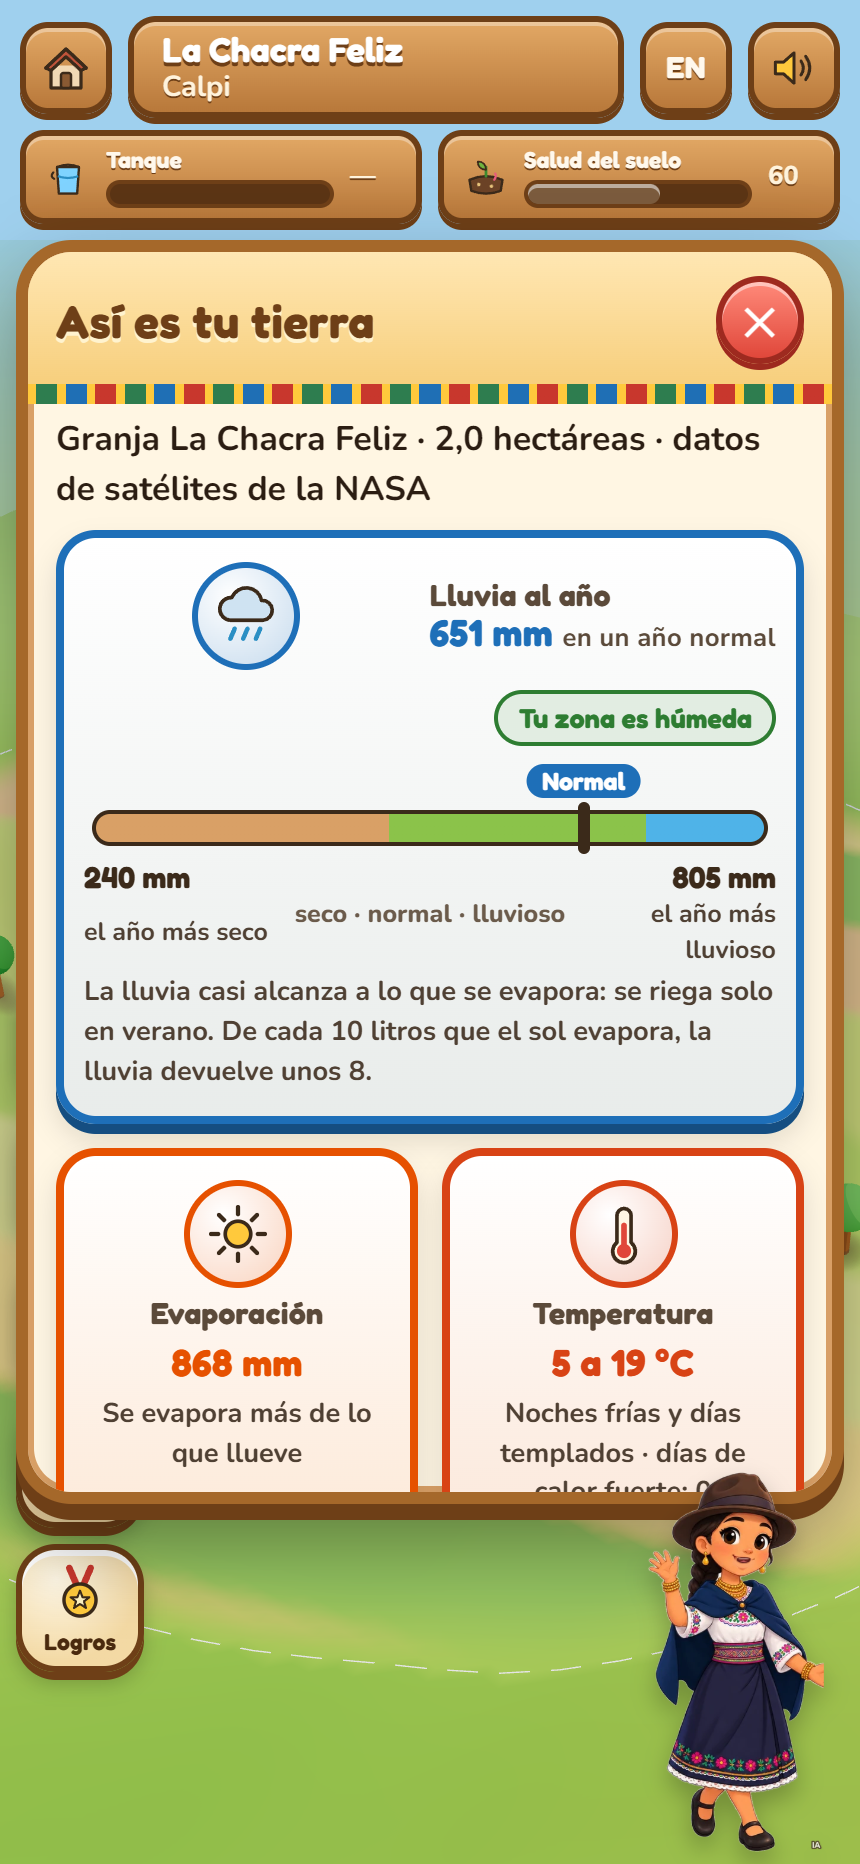
\includegraphics[height=8.3cm]{../capturas/ficha_es.png}\hfill
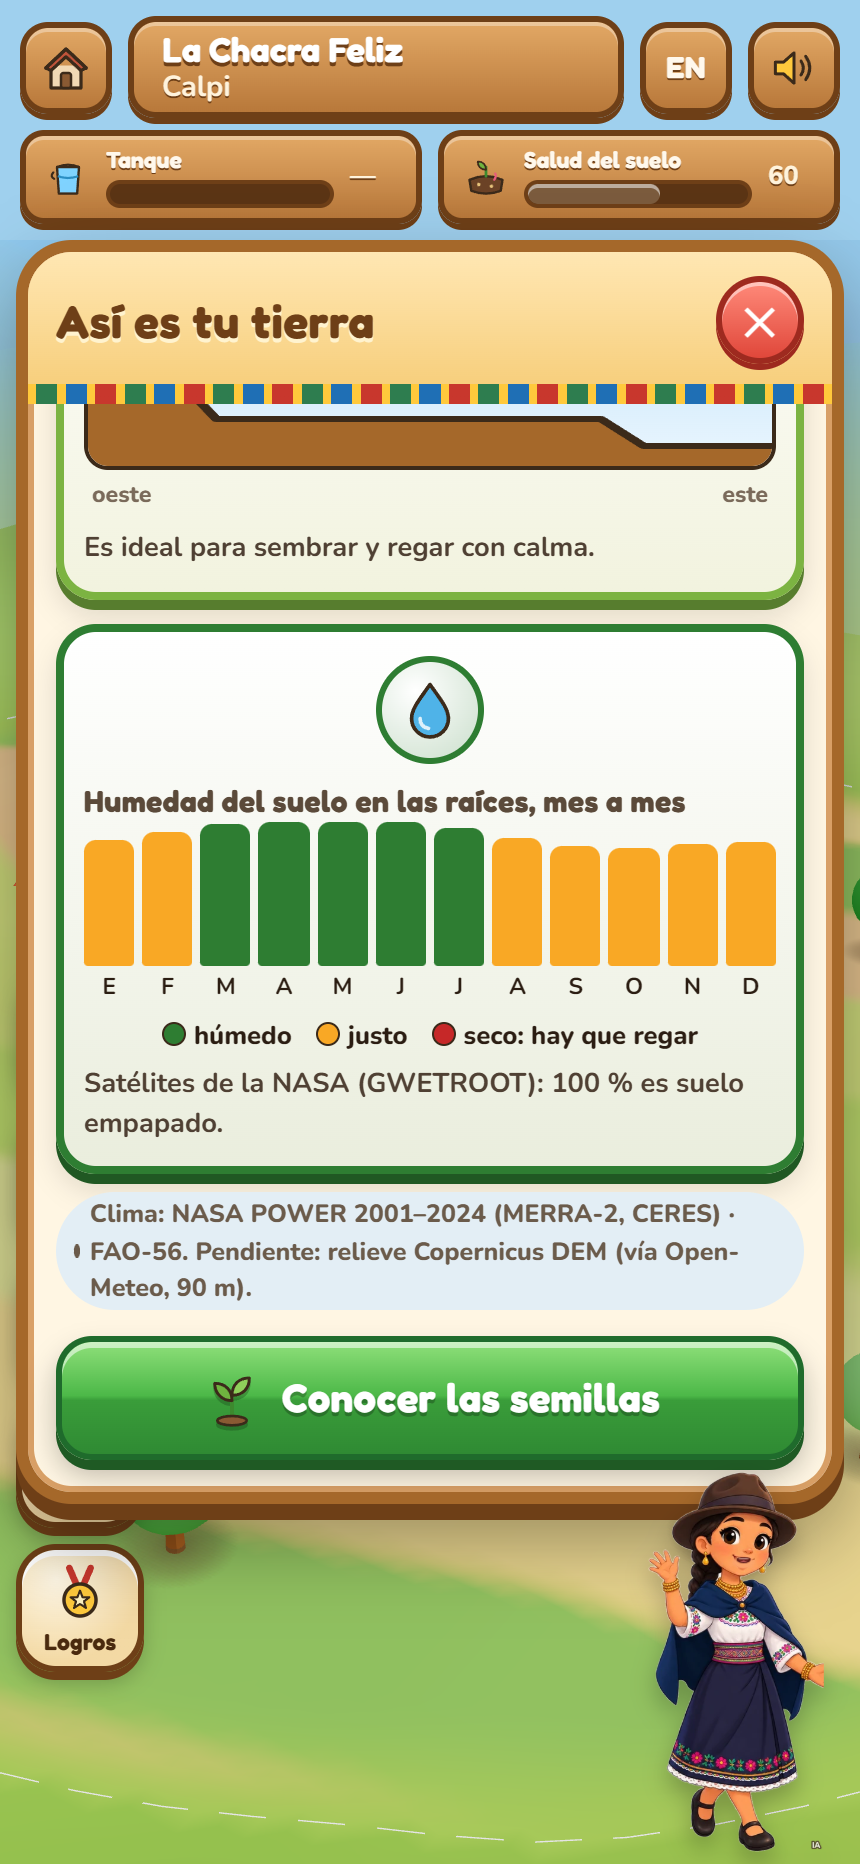
\includegraphics[height=8.3cm]{../capturas/ficha2_es.png}\hfill
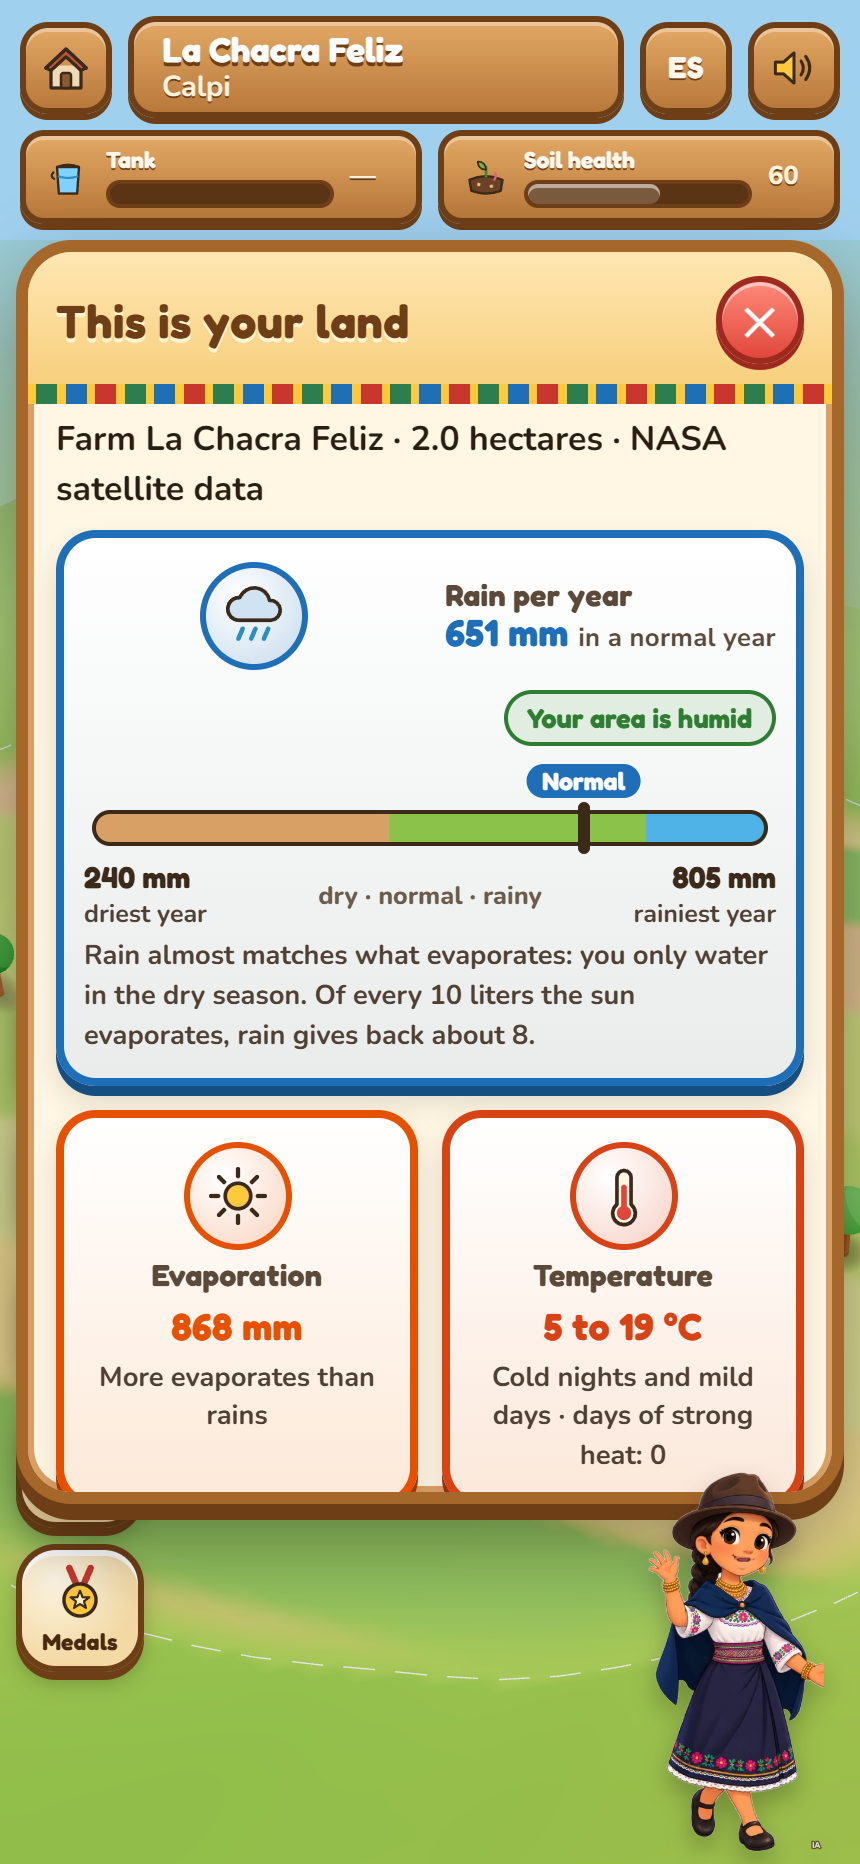
\includegraphics[height=8.3cm]{../capturas/ficha_en.png}\\[3pt]
{\footnotesize Izquierda: rango de lluvia anual (año más seco 240 mm, normal 651 mm, más lluvioso 805 mm) e índice de aridez.
Centro: humedad del suelo en las raíces (GWETROOT) mes a mes. Derecha: la misma ficha en inglés.
Pachita e íconos de cultivos: imágenes generadas con IA.}
\end{tarjeta}

%=============================== ENGLISH ===============================
\begin{otherlanguage}{english}
\banda{Astro Granja}{Project fact sheet · A kids' farming game powered by real NASA data}%
{\textbf{Aquarela Team} · Challenge \textbf{Field Shift: Adapting Farms with NASA Data} · NASA Space Apps Challenge 2026 · Sangolquí (ESPE), Ecuador}

\begin{tarjeta}{High-level summary}
Astro Granja turns open NASA POWER data into a farming game for children in the Ecuadorian Andes. Pachita, an Andean farmer,
helps kids pick their real plot on a map, read its climate from NASA satellites, plant Andean crops in season, water only when
the soil is thirsty and rotate with nitrogen-fixing legumes so the soil recovers.
\end{tarjeta}

\begin{tarjeta}[azul]{Project details}
\small
\textbf{Problem.} Highland smallholders repeat potato season after season, the soil loses nutrients, and rainfall is becoming harder
to predict. Children in rural schools are the next generation of farmers but rarely see climate data explained for their own land.\\[2pt]
\textbf{Approach.} A FastAPI science engine (Python) downloads 24 years of daily NASA POWER data for the chosen point, fills gaps,
corrects rain and temperature for altitude, computes FAO-56 Penman-Monteith evapotranspiration and a daily soil-water balance per
crop, and ranks rotations. A mobile web game (Astro + three.js, with a no-3D mode) turns those numbers into a story.\\[2pt]
\textbf{What we built.} Rocket landing, real-plot map, a “This is your land” sheet with NASA rain range, temperature, sunlight,
humidity and GWETROOT soil moisture; seeds grouped by botanical family; planting calendar; 3D farm where each day uses that
place's real weather; drought and heat stress, watering in liters, harvest, crop rotation and a certificate. Spanish and English.\\[2pt]
\textbf{Results and next steps.} Working prototype deployed at pacha-chat.vercel.app; demo sites work offline. Next: test with
rural schools and water boards, add Kichwa voice, and more satellite soil data.
\end{tarjeta}

\begin{tarjeta}[verde]{NASA data · Links · AI}
\small
\textbf{NASA data:} \enlace{https://power.larc.nasa.gov/docs/services/api/temporal/daily/}{NASA POWER Daily API}
(PRECTOTCORR, T2M\_MAX, T2M\_MIN, RH2M, WS2M, ALLSKY\_SFC\_SW\_DWN; 2001–2024) and
\enlace{https://power.larc.nasa.gov/docs/services/api/temporal/climatology/}{NASA POWER Climatology API} (GWETROOT, GWETTOP),
built on \enlace{https://gmao.gsfc.nasa.gov/reanalysis/MERRA-2/}{MERRA-2}, \enlace{https://ceres.larc.nasa.gov/}{CERES} and
\enlace{https://gpm.nasa.gov/data/imerg}{GPM IMERG}.\\[2pt]
\textbf{Links:} demo \enlace{https://pacha-chat.vercel.app}{pacha-chat.vercel.app} ·
code \enlace{https://github.com/M47H3W1/pacha-bot}{github.com/M47H3W1/pacha-bot} (\enlace{https://github.com/M47H3W1/pacha-bot/blob/develop/LICENSE}{MIT License}).\\[2pt]
\textbf{AI disclosure:} code written with Claude Code and reviewed and tested by the team; Pachita and crop images are AI-generated
and marked “IA”; Pachita's voice uses edge-tts. Data and calculations were validated by the team. No NASA logos were generated or altered.
\end{tarjeta}

\vfill
{\footnotesize\color{tierra!80} Team: Nikol Montiel (research), Mathew Gutiérrez (AI \& data), Santiago Rubio (design), Miguel Ávilez (development).}
\end{otherlanguage}

\end{document}
